\documentclass[twocolumn,twoside,10pt,nodate]{article}
\usepackage{amsmath,amssymb}
\usepackage{fancyhdr}
\usepackage{graphicx}% Include figure files
\usepackage[english]{babel}
\usepackage{hyperref}

\newcommand{\titolo}[2]{\title{\Large\bf\vspace{-1cm}#1}}
%\newcommand{\website}[1]{\newcommand{\site}{#1}}

\setlength\oddsidemargin{-.2cm}
\setlength\evensidemargin{-1.1cm}
\setlength\textwidth{17.5cm}
\setlength\topmargin{-2cm}
\setlength\textheight{25cm}

\begin{document}

% ** Please do NOT remove/change anything above this line **** 

\titolo{Search for new long-lived particles at LHC with the CMS detector}

\date{}%  ** do NOT remove this line **
\maketitle
\thispagestyle{fancy} % ** do NOT remove this line **

Extensions of the Standard Model (SM) predict the existence of new
particles which can be created in high-energy proton-proton (pp) 
collisions at the LHC. The lifetime of these new massive states is
often a free parameter of the theory. 
%The new particle might be so
%short-lived that it decays  within a microscopic distance of the place
%where it was created, 
%The new particle decay promptly after production, in which case the 
%new state can only be inferred by studying its decay products. 
%This is how the majority of searches for new physics are performed at
%LHC. Alternatively, 
If the new particle is long-lived, it will decay far from the pp
interaction point and can interact directly with the detector while
traveling thought it. The experimental signatures of long-lived
particles (LLPs) are usually striking but also very different from 
the short-lived ones, thus requiring dedicated analysis methods.

Searches for LLPs have been performed in a
wide range of final states with the CMS detector 
and, so far, no evidence of these signals have been found.
%significant deviations from the SM
%expectations have been observed. 
The CMS collaboration published 
15 papers on this topic [1]. A large number of experimental 
signatures has been explored, as outlined in Fig. 1, including:

\begin{figure}[h]
\centering
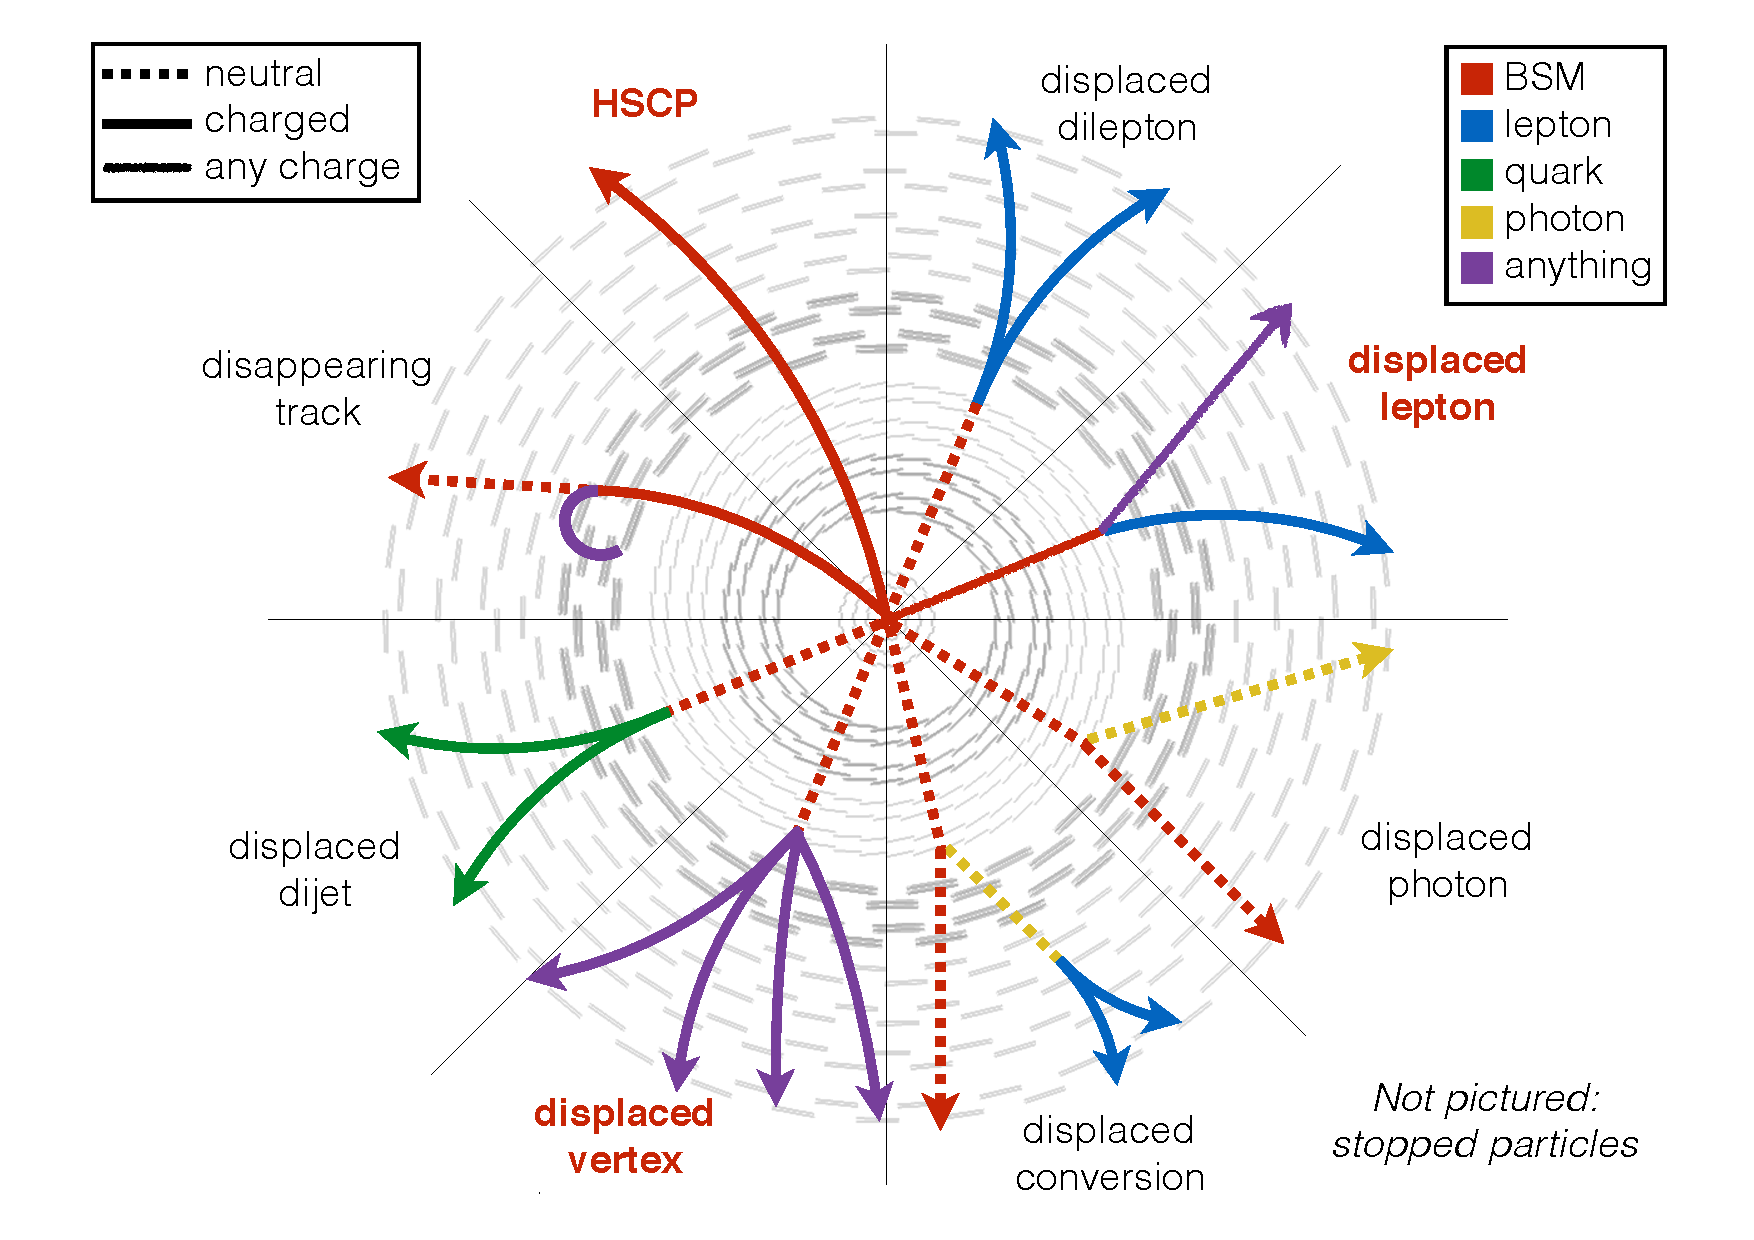
\includegraphics[width=0.45\textwidth,angle=0]{santanastasio_fig1.pdf}
\caption{\small Experimental signatures of new long-lived particles (LLPs) 
in the CMS detector. LLPs are indicated with the label BSM (beyond the Standard Model).} % Please do NOT change the caption style
\end{figure}

\begin{itemize}
\item {\bf Heavy Stable Charged Particles (HSCP)}: at LHC these massive 
particles are typically produced with $\beta$ significantly less than
1. They can be
%mass greater than 100
%GeV, non-relativistic ($\beta<1$), lifetime greater than a few
%nanoseconds, in some cases charge not equal to $\pm e$. 
identified by unusual rate of energy loss via ionization in the inner
tracker material or through their 
%longer 
longer time-of-flight to the outer tracking detectors
compared to light SM particles (such as muons). 
Recent results are reported in Ref.[2];
\item {\bf Stopped particles}: slow HSCPs ($\beta \ll 1$) can lose all 
their momentum via ionization and stop in the calorimeters. 
  Their decays can be detected out-of-time with respect to the
  LHC collisions, even hours or days after the pp collision that produced
  them;
\item {\bf Displaced vertices}: the LLP can be a neutral particle
  decaying into SM charged particles (hadrons or leptons) within the
  inner tracker volume. They can be identified via the reconstruction
  of decay vertices displaced from the pp interaction point;
\item {\bf Disappearing tracks}: a disappearing-track signature can be produced by a
  charged LLP whose decay products are undetected;
%Disappearing tracks 
%are identified as those with little or no associated calorimeter
%energy deposits and with missing hits in the outer layers of the tracker;
\item {\bf Displaced photons}: a neutral LLP can decay to a photon and a weakly
  interacting particle. 
%(the latter evades detection). 
The photon arrival at
  the electromagnetic calorimeter (ECAL) is delayed, due to extra flight
  length added by the LLP decay. This time delay, unusual for photons
  generated by SM processes, can be measured taking advantage of the
  excellent ECAL time resolution. Displaced photons are foreseen for
  example by neutralino decays in Supersymmetry. 
%(SUSY) models with gauge mediated
%  SUSY breaking. 
The first search in CMS was performed by the Rome group using data at
$\sqrt{s}=7$~TeV and no deviation from the SM predictions was found [3].
Limits were set on the neutralino mass as a function of its proper
decay length, as shown in Fig. 2, extending results from previous experiments.
\end{itemize}

\begin{figure}[h]
\centering
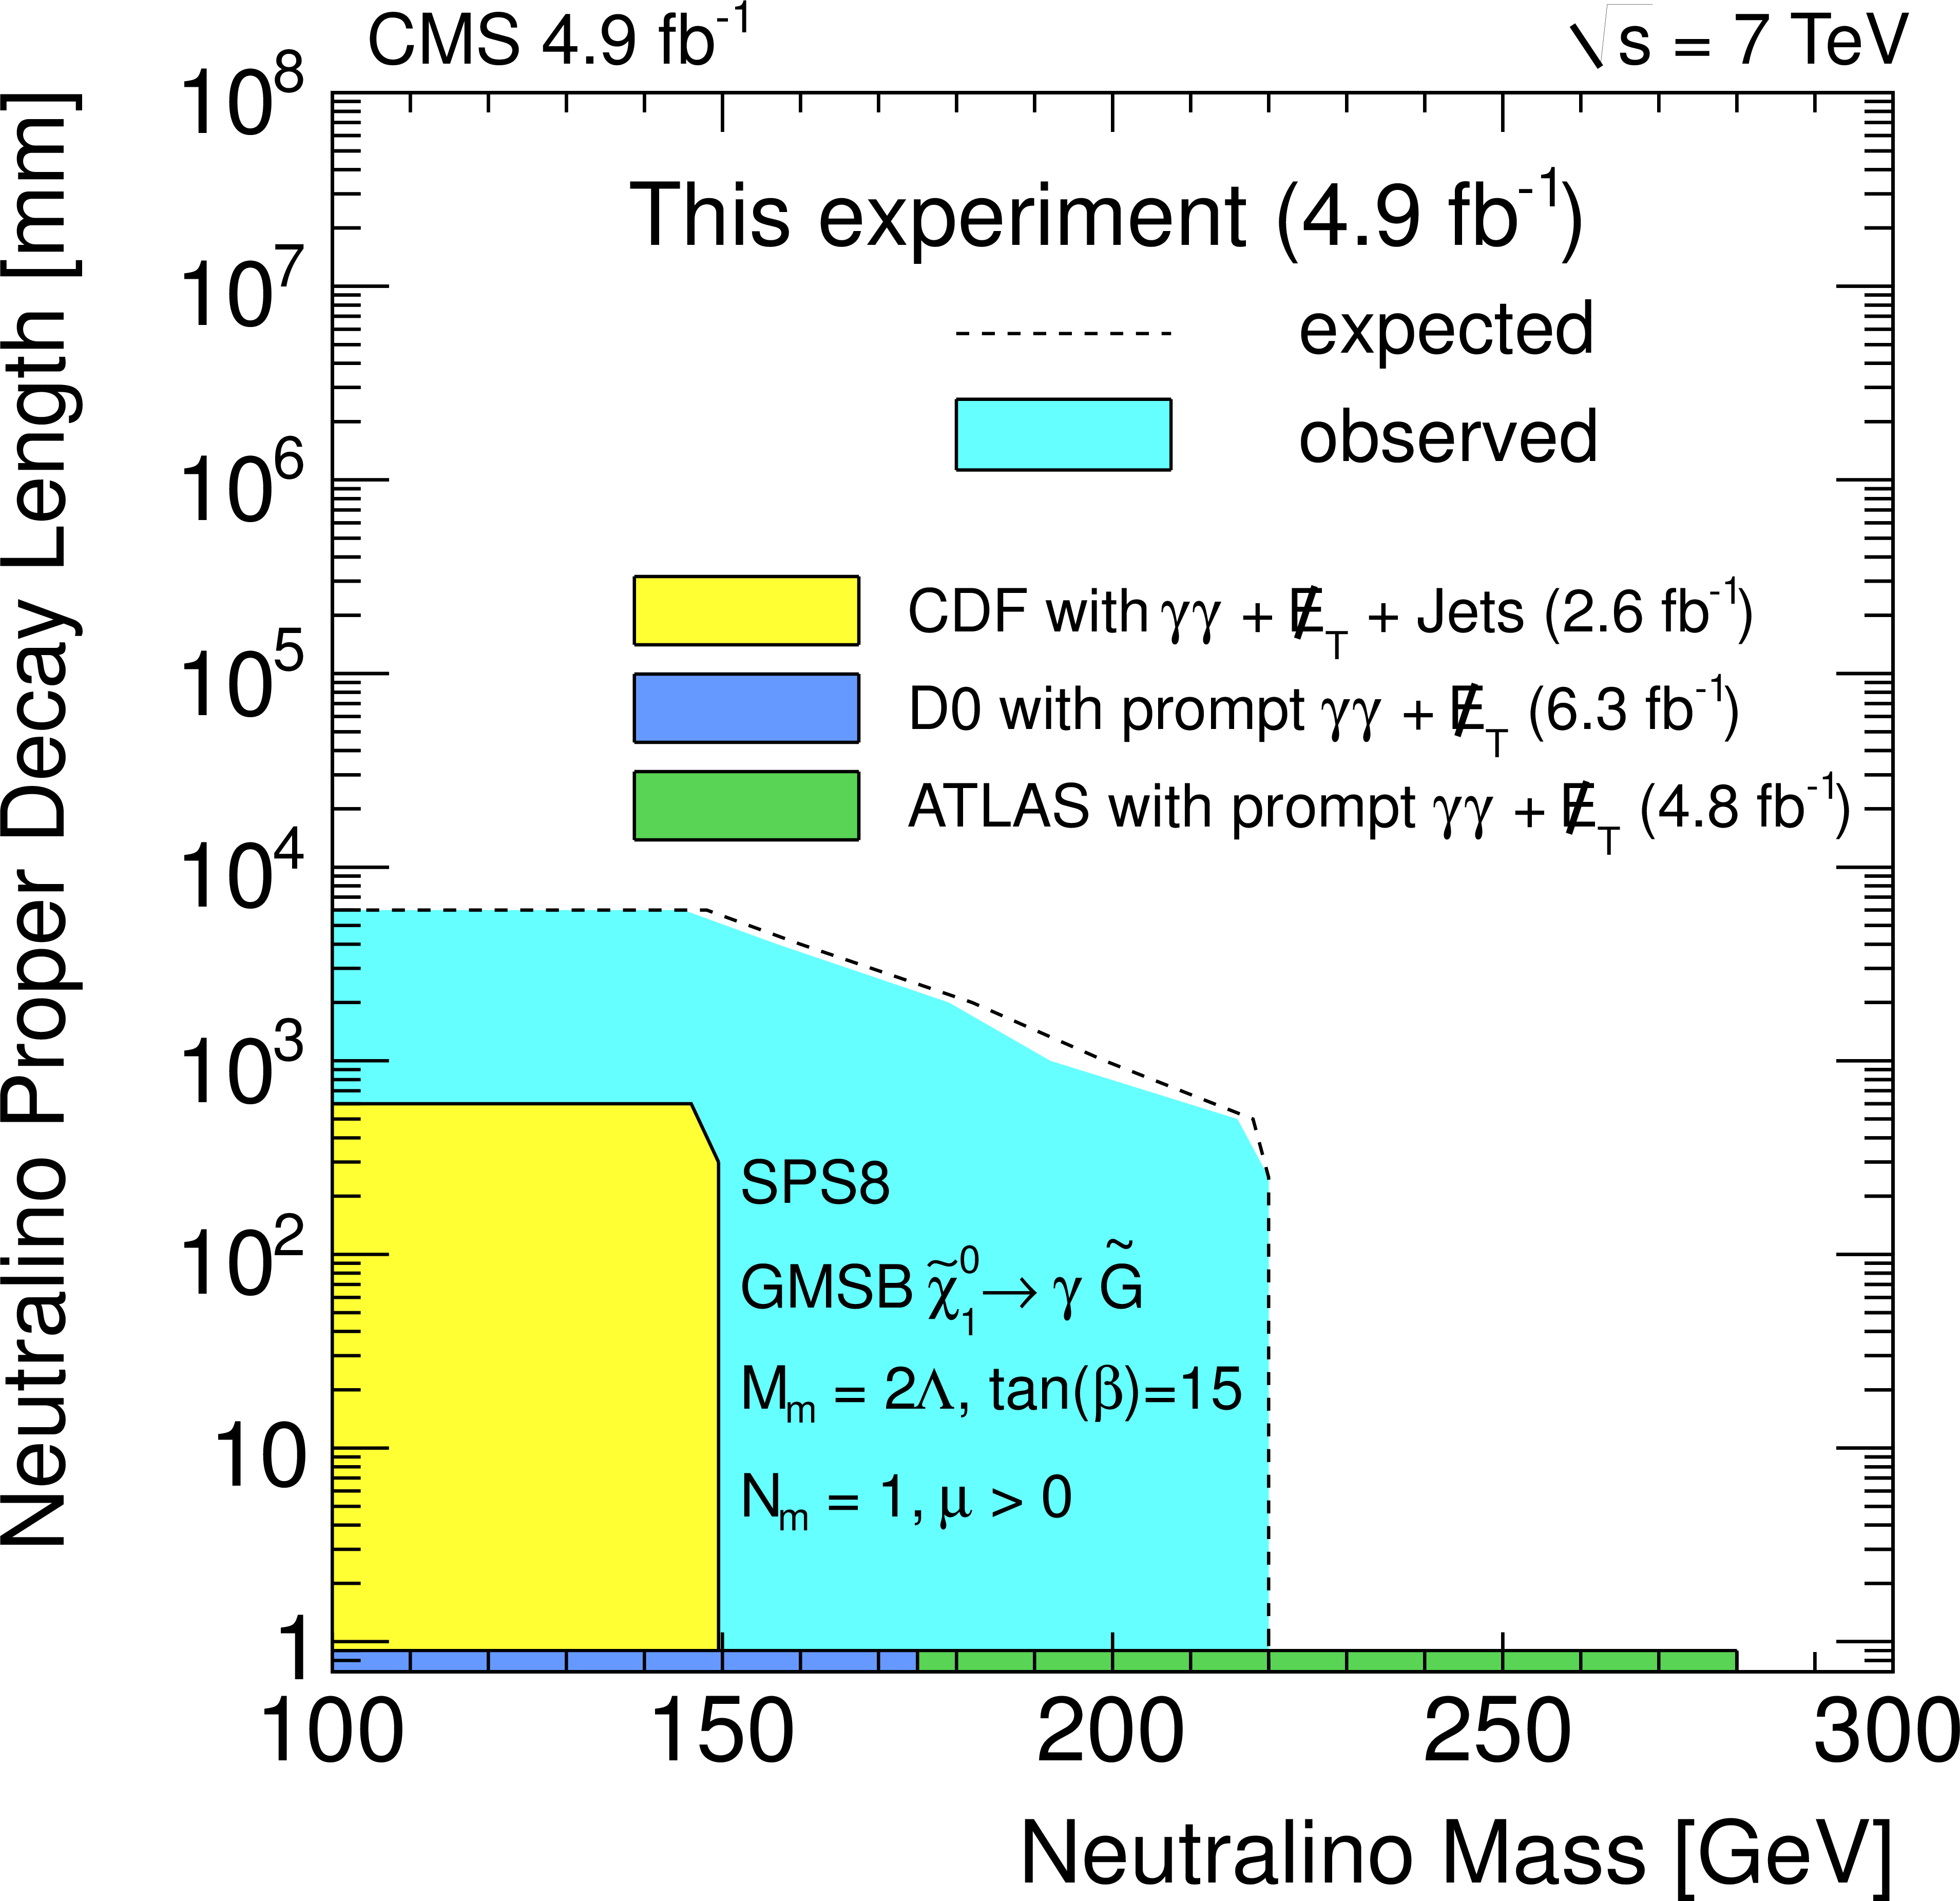
\includegraphics[width=0.30\textwidth,angle=0]{santanastasio_fig2.png}
\caption{\small Excluded regions in the neutralino proper decay length
  ($c\tau$) vs mass plane.} % Please do NOT change the caption style
\end{figure}

%The discussion has started in view of the upgrade of the detectors for
%the phase of higher LHC luminosities. The search for long-lived
%particles has to be taken in account in designing the upgraded
%detectors, since their reconstruction capabilities have to be
%preserved, as well as dedicated trigger algorithms to 
%identify such signatures.

%\begin{itemize}
%\item theory intro
%\item status of CMS searches
%\item list of most important final states
%\item two example of searches done at Rome, or associated to
% activities in Rome
%\end{itemize}


%\begin{itemize}
% \item The filename should be \url{last_name_of_the_main_contributor.tex}, as in \url{fermi.tex}.
% \item Any acronym should be introduced at its first occurrence;
% \item Figures can be included in the standard way, cf. Fig.~1. \url{.pdf} format is preferred, but also \url{.eps} and \url{.png} can be used. 
% \item The name of the $N$-th figure should be \url{last_name_of_the_main_contributor_figN.pdf}, as in \url{fermi_fig1.pdf};
% \item Tables can be also included as in Table~1;
% \item References (max~$4$) can be introduced as in [1] and should be numbered in order of their appearance [2];
% \item Please note the reference style: First Author \textit{et al.}, Journal \ \textbf{Volume} Page (Year)
% \item For bibliographic entries with $4$ or more authors\footnote{The complete list of authors will be available in the final section of the Scientific Report, together with the complete list of publications affilated to the Physics Department.}, please use ``\textit{et al.}'' as in [1];
% \item The Authors list appears at the end of the document and contains the list of people (including researchers, postdoc, PhD students) involved in the research described by the contribution;
% \item If one of the authors is not a member of the Physics Department but is affiliated to external institutions (e.g., CNR, INAF, INFN, etc), please use the mark as in E.~Amaldi$^X$ in the author list below;  During the post-processing, we will take care of writing the correct affiliation number, which will appear in a different page;
% \item Please select the corresponding Subject Area: Theoretical Physics,Particle Physics, Condensed Matter Physics, Biophysics, or Astronomy, Astrophysics \& Geophysics.
%\end{itemize}

%\begin{figure}[h]
%\centering
%
\includegraphics[width=0.45\textwidth,angle=0]{template_fig1.pdf}
%\caption{\small
%Entrance of the Department's main building [1].} % Please do NOT change the caption style
%\end{figure}

%%%%%%%%%%%%%
%\begin{table}[htbp]
%	\centering
% \begin{tabular}{|c|r|r|r|} 
% \hline
%          A               & B             & C                              \\
%          A               & B             & C                              \\
%          A               & B             & C                              \\
%          A               & B             & C                              \\
%  \hline
%  \end{tabular}
%	\caption{Template of a table.}
%\end{table}	


%%%
%%%%
% \\
% \\
%%%%%%%%
% Please do NOT remove the following two lines
% \\
% \\
%%%%%
\vfill
\small{
\noindent
\textbf{References}
\\
1. \url{http://cms-results.web.cern.ch/cms-results/public-results/publications/EXO/LLP.html}\\
2. The CMS Collaboration, Phys. Rev. D \ \textbf{94} 112004 (2016) \\
%\href{https://arxiv.org/abs/1609.08382}{arXiv:1609.08382} (2016) \\
3. The CMS Collaboration, Phys. Lett. B \ \textbf{722} 273 (2013)
%2. E.~Fermi, E.~Amaldi, Journal \ \textbf{Volume} Page (Year). 
%%%%
% Please do NOT remove the following two lines
\\
\\
\noindent
\textbf{Authors}
\\
L.M. Barone, F. Cavallari$^X$, D. Del Re, M. Diemoz$^X$, E. Di Marco$^X$ , E. Longo, P. Meridiani$^X$ ,G. Organtini, R. Paramatti, S. Rahatlou, C. Rovelli$^X$ , F. Santanastasio.
%N. Template, E. Fermi, E.~Amaldi$^X$
\\
\\
\url{http://cms.web.cern.ch/}
\\
\\
\noindent
\textbf{Subject Area}
\\
%Template
%
% Please choose one by removing the comment in the text:
%
% Theoretical Physics 
Particle Physics
% Condensed Matter Physics
% Biophysics
% Astronomy, Astrophysics \& Geophysics 
%
}
\end{document}
